\documentclass[aspectratio=1610]{beamer}
\usepackage[utf8]{inputenc}
\usepackage[T1]{fontenc}
\usepackage[german]{babel}
\usepackage[useregional]{datetime2}
\usepackage[nameinlink]{cleveref}
\usepackage[section]{placeins}
\usepackage{xcolor}
\usepackage{graphicx}
\usepackage{csquotes}
\usepackage{amsmath} % for $\text{}$
\usepackage{enumitem}
\usepackage{abschluss}
\usepackage{algorithm}
\usepackage{algorithmicx}
\usepackage{algpseudocode}
\usepackage{listings}
\usepackage{bera}
\usepackage{pdfpages}
\usepackage{colortbl}
\usepackage{chronosys}
\usepackage{tikz}
\usetikzlibrary{trees}

\colorlet{punct}{red!60!black}
\definecolor{background}{HTML}{EEEEEE}
\definecolor{delim}{RGB}{20,105,176}
\colorlet{numb}{magenta!60!black}
\lstdefinelanguage{json}{
    basicstyle=\normalfont\ttfamily,
    numbers=left,
    numberstyle=\scriptsize,
    stepnumber=1,
    numbersep=8pt,
    showstringspaces=false,
    breaklines=true,
    frame=lines,
    backgroundcolor=\color{background},
    literate=
     *{0}{{{\color{numb}0}}}{1}
      {1}{{{\color{numb}1}}}{1}
      {2}{{{\color{numb}2}}}{1}
      {3}{{{\color{numb}3}}}{1}
      {4}{{{\color{numb}4}}}{1}
      {5}{{{\color{numb}5}}}{1}
      {6}{{{\color{numb}6}}}{1}
      {7}{{{\color{numb}7}}}{1}
      {8}{{{\color{numb}8}}}{1}
      {9}{{{\color{numb}9}}}{1}
      {:}{{{\color{punct}{:}}}}{1}
      {,}{{{\color{punct}{,}}}}{1}
      {\{}{{{\color{delim}{\{}}}}{1}
      {\}}{{{\color{delim}{\}}}}}{1}
      {[}{{{\color{delim}{[}}}}{1}
      {]}{{{\color{delim}{]}}}}{1},
}

\setlist{nosep}

\newcommand\urlpart[2]{$\underbrace{\text{\texttt{#1}}}{\text{#2}}$}
\raggedbottom
\crefname{figure}{Abb}{Abb}

\newcommand\producttitle{treff.}
\hypersetup{
	pdftitle={Qualitätssicherungsphase: \producttitle},
	bookmarks=true,
}

% header & footer
\usepackage{scrlayer-scrpage}
%\lofoot{\today}
%\refoot{\today}
\pagestyle{scrheadings}

\title{
\includegraphics[width = 50mm]{images/logo_crop.png}}
\subtitle{\huge Abschlusspräsentation}
\author{Lukas Dippon
	\and Jens Kienle
	\and Matthias Noll
    \\Fabian Röpke
	\and Tim Schmidt
	\and Simon Vögele}

\begin{document}

	\begin{frame}[plain]
	\maketitle
	\end{frame}

%%%%%%%% Idee/Vision %%%%%%%%%%

	\begin{frame}[plain]
      \frametitle{\textbf{Aufgabenstellung}}
      \begin{itemize}
        \item[--] Entwicklung einer Android App
        \item[--] Verwendung einer Client-Server Architektur
        \item[--] Inspiration durch "Go-App"
        \item[--] App zum Koordinieren kleiner Personenkreise
        \item[--] Keine closed source dependencies
        \item[--] Kein Ungewolltes Tracking
        \item[--] Kein Social Network
      \end{itemize}
  \end{frame}

  \begin{frame}[plain]
      \frametitle{\textbf{Datenmodell}}
      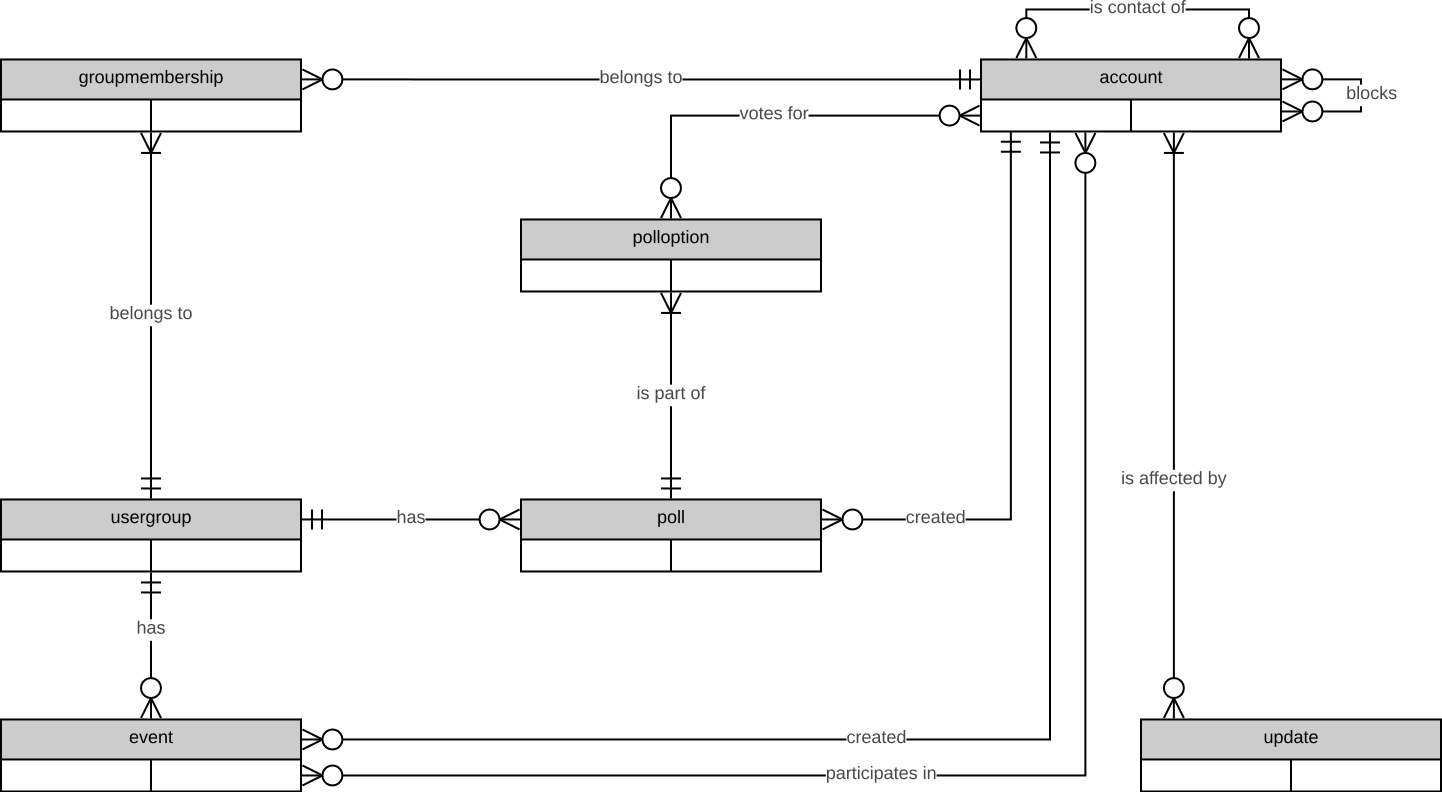
\includegraphics[width = \columnwidth - 30pt]
        {images/erd.png}
      %TODO ggf auf anderem Bildschirm zeitgleich mit der Folie davor?
      %TODO andere Darstellung
  \end{frame}

%%%%%%%% Umsetzung %%%%%%%%%%

  \begin{frame}[plain]
      \frametitle{\textbf{Arbeitsweise - Arbeitsaufteilung}}
      \begin{itemize}
          \setlength\itemsep{0.3em}
          \item[--] 3 Personen für den Klient
              \begin{itemize}
                  \item[--] Fabian
                  \item[--] Lukas
                  \item[--] Matthias
              \end{itemize}
          \item[--] 3 Personen für den Server
              \begin{itemize}
                  \item[--] Jens
                  \item[--] Simon
                  \item[--] Tim
              \end{itemize}
      \end{itemize}
  \end{frame}

  \begin{frame}[plain]
      \frametitle{\textbf{Arbeitsweise - Tools}}
      \begin{minipage}{0.45\textwidth}
        \begin{itemize}
          \item[--] GitHub
          \item[--] LaTeX
          \item[--] IntelliJ/AndroidStudio
          \item[--] Kanban board \& Etherpad
          \item[--] PlantUML
        \end{itemize}
      \end{minipage}
      \begin{minipage}{0.45\textwidth}
        
\includegraphics[width = \columnwidth - 30pt]
          {images/tools.png}
      \end{minipage}
  \end{frame}

  \begin{frame}[plain]
      \frametitle{\textbf{Arbeitsweise - Kommunikation}}
      \begin{minipage}{0.45\textwidth}
        \begin{itemize}
          \item[--] Telegram
          \item[--] Discord \& TS
          \item[--] Persönliche Treffen \\ v.a. zwischen Vorlesungen
        \end{itemize}
      \end{minipage}
      \begin{minipage}{0.45\textwidth}
        
\includegraphics[width = \columnwidth - 30pt]
          {images/meet-im-voip.png}
      \end{minipage}
  \end{frame}

  \begin{frame}[plain]
      \frametitle{\textbf{Server -- Struktur}}
      % TODO: Knappe Übersicht über Command Design, Interfaces- und SQL-Package
      TODO
  \end{frame}

  \begin{frame}[plain]
        \frametitle{\textbf{Server} -- Locking und Deadlocks}
        \only<1>{
            \begin{figure}
                \footnotesize
                \startchronology[startyear=1,stopyear=50,dates=false,
                width=0.9\textwidth]
                \chronoevent{1}{\code{call execute()}}
                \chronoevent[markdepth=30pt]{8}{\code{readLock(x)}}
                \chronoevent{13}{\code{x.getFoo()}}
                \chronoevent{32}{\code{x.getBar()}}
                \chronoevent[markdepth=30pt]{38}{\code{releaseReadLock(x)}}
                \chronoperiode[color=cyan]{8}{38}{Crit. Section}
                \stopchronology
                \caption{Thread 1}
            \end{figure}
            \vspace{-30pt}
            \begin{figure}
                \footnotesize
                \startchronology[startyear=1,stopyear=50,dates=false,
                arrowcolor=cyan,width=0.9\textwidth]
                \chronoevent{1}{\code{call execute()}}
                \chronoevent[markdepth=30pt]{14}{\code{writeLock(x)}}
                \chronoevent[markdepth=30pt]{39}{\code{x.setFoo(2)}}
                \chronoperiode[color=orange]{14}{38}{Blocked}
                \chronoperiode[color=cyan]{38}{50}{Crit. Section}
                \stopchronology
                \caption{Thread 2}
            \end{figure}
        }
        \only<2>{
            \begin{minipage}{.5\textwidth}
                \textbf{Locking order}
                \begin{itemize}
                    \item[1.] Von oben nach unten in der\\Zugriffshierarchie
                    \item[2.] Usergroups vor Updates;\\Events vor Polls
                    \item[3.] Niedrige IDs vor hohen IDs
                \end{itemize}
            \end{minipage}%
            \begin{minipage}{.5\textwidth}
                \begin{figure}
                    \begin{tikzpicture}[level distance=1.5cm,
                        level 1/.style={sibling distance=3cm},
                        level 2/.style={sibling distance=1.5cm}]
                        \node{Account}
                                child {node {Usergroup} edge from parent[->]
                                child {node {Event}}
                                child {node {Poll}
                                    child {node {PollOption}}
                                }
                            }
                            child {node {Update} edge from parent[->]};
                    \end{tikzpicture}
                    \caption{Zugriffshierarchie}
                \end{figure}
            \end{minipage}
        }
        \only<3>{
            \begin{figure}
                \footnotesize
                \startchronology[startyear=1,stopyear=50,dates=false,
                arrowcolor=red,width=0.9\textwidth]
                \chronoevent{1}{\code{call execute()}}
                \chronoevent[markdepth=30pt]{13}{\code{readLock(x)}}
                \chronoevent{25}{\code{Set s = \{u,v,w,x,y,z\}}}
                \chronoevent[markdepth=30pt]{40}{\code{writeLockAllInSet(s)}}
                \chronoperiode[color=cyan]{13}{22}{Crit. Section}
                \chronoperiode[color=red,dates=false]{40}{50}{Deadlock}
                \stopchronology
                \caption{Deadlocks auch bei $\vert Threads\vert = 1$}
            \end{figure}
        }
        \only<4-5>{
            \begin{figure}
                \begin{tabular}{ c | c | c }
                    \textbf{Test \#} & \textbf{Run \#} & \textbf{Result} \\
                    \hline
                    1 & 1 & \cellcolor{green!25}Works \\
                    1 & 2 & \cellcolor{green!25}Works \\
                    1 & 3 & \cellcolor{gray!25}Doesn't terminate \\
                    1 & 4 & \cellcolor{green!25}Works \\
                    1 & 5 & \cellcolor{gray!25}Doesn't terminate \\
                \end{tabular}
                \caption{Effektivität von Concurrency-Tests hängt vom Scheduler
                ab}
            \end{figure}
        }
        \only<5>{
            \centering{Kein Compiler-Fehler/-Warnung und nicht reproduzierbar
            im Debugger}\\
            \centering{$\implies$ Statische Analyse nötig}
        }
        \only<6>{
            \begin{figure}
                \footnotesize
                \startchronology[startyear=1,stopyear=50,dates=false,
                arrowcolor=orange,width=0.9\textwidth]
                \chronoevent{1}{\code{call execute()}}
                \chronoevent[markdepth=45pt]{13}{\code{readLock(x)}}
                \chronoevent[markdepth=15pt]{22}{\code{releaseReadLock(x)}}
                \chronoevent[markdepth=45pt]{30}{\code{Set s = new HashSet()}}
                \chronoevent[markdepth=15pt]{40}{%
                    \code{writeLockAllInSet(s)}}
                \chronoperiode[color=cyan]{13}{22}{Crit. Section}
                \chronoperiode[color=orange,dates=false]{40}{50}{Pot. Deadlock}
                \stopchronology
                \caption{Deadlocks durch falsche Locking-Order}
            \end{figure}
        }

    \end{frame}

  \begin{frame}[plain]
      \frametitle{\textbf{Interessante Stellen - Client}}
      %TODO osmdroid (clustering etc)
  \end{frame}

  \begin{frame}[plain]
      \frametitle{\textbf{Probleme}}
      \begin{itemize}
        \item[--] Arbeitsaufwand unterschätzt
        %TODO LoC-Graph auf anderem Bildschirm
        \item[--] Teilweise schlechtes Zeitmanagement
        %TODO Phasengrenzen in LoC-Graph einblenden
        \item[--] Zu wenig Leute beim Client
        \item[--] Aufteilung in Teams => mangelnde Kommunikation
        \item[--] Zu wenig Gedanken über Implementierung im Entwurf
        \item[--] Zu wenig Gedanken über Qualitätssicherung bei der Implementierung
      \end{itemize}
  \end{frame}

%%%%%%%% Ergebnis %%%%%%%%%%

  \begin{frame}[plain]
      \frametitle{\textbf{Demo}}

  \end{frame}

  \begin{frame}[plain]
      \frametitle{\textbf{Erweiterungsmöglichkeiten}}
        \begin{itemize}
          \item[--] Abstimmungen
          \item[--] Gruppenrollen und -rechte
          \item[--] Detaillierte Innenraumkarten
          \item[--] Stummschalten
          \item[--] Zeitplan für Positionsübertragung
          \item[--] Passwortzurücksetzung
          \item[--] Profil- und Gruppenbilder
          %TODO Bilder auf dem anderen Bildschirm?
        \end{itemize}
        %TODO unerfüllte Kür
        %TODO Erfülltheitstabelle:
        % Features x (Server-Impl., Server-Getestet, Client-Impl., Client-Test)
  \end{frame}

\end{document}
